\documentclass{article}

\usepackage{a4wide}
\usepackage[utf8]{inputenc}
\usepackage[T1]{fontenc}
\usepackage[french]{babel}
\usepackage[babel=true]{csquotes}
\usepackage{graphicx}
\graphicspath{{Image_projet/}}
\usepackage{color}
\usepackage{hyperref}
\hypersetup{colorlinks,linkcolor=,urlcolor=blue}

\usepackage{amsmath}
\usepackage{amssymb}


\title{Rapport du jeu Escape From Space de FOCKING Vincent et HUBERT Gregory}
\author{Vincent Focking et Grégory Hubert, L3 informatique}

\begin{document}

\maketitle


\begin{abstract}
  Dans ce rapport nous vous présenterons le jeu mobile que nous avons créé dans le cadre du projet de développement mobile. Notre jeu Escape From Space nous invite à diriger un vaisseau dans l'espace afin qu'il évite les météores qui pourraient le toucher. En reprenant les anciens mode de jeu sous le culte du High Score nous faisons en sorte que vous donniez le meilleur de vous même  et faire en sorte que le vaisseau aille le plus loin possible. Le jeu a un gameplay et affichage quasi identique sur les deux plateformes cependant nous voulions différencier un peu les deux applications en modifiant quelques petites mécaniques (expliquer plus tard dans le rapport) qui montre des manières différentes de coder le jeu. \LaTeX.
\end{abstract}


\section{Introduction}

Nous vous présenterons l'application de manière général afin de voir toutes les fonctionnalités qu'elle propose. 
Puis nous verrons plus en profondeur le code Android et IOS de cette même application pour ensuite conclure sur ce que ce projet nous a apporté.


\section{Description générale de l'application}

\subsection{Le Menu} 
\begin{minipage}[c]{.46\linewidth}
     \begin{center}
             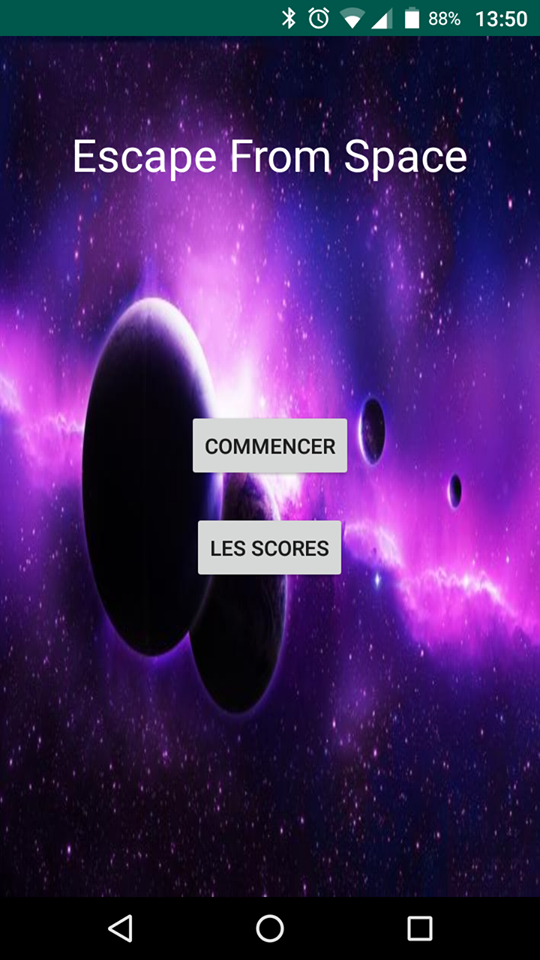
\includegraphics[scale=0.2]{Menu.png}
         \end{center}
   \end{minipage} \hfill
   \begin{minipage}[c]{.46\linewidth}
    \begin{center}
            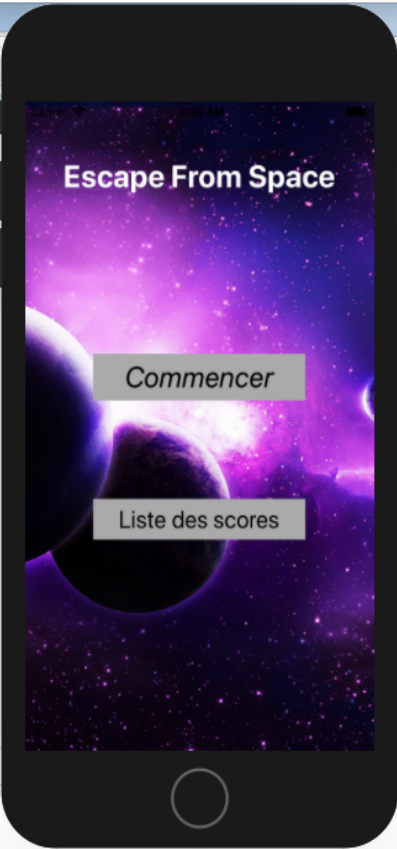
\includegraphics[scale=0.38]{MenuIOS.png}
        \end{center}
 \end{minipage}


Ici nous voyons un menu basique avec le titre du jeu, deux boutons qui amène l'un à commencer le jeu et l'autre vers l'écran de score.

\subsection{Prêt à jouer} 
\begin{center}
 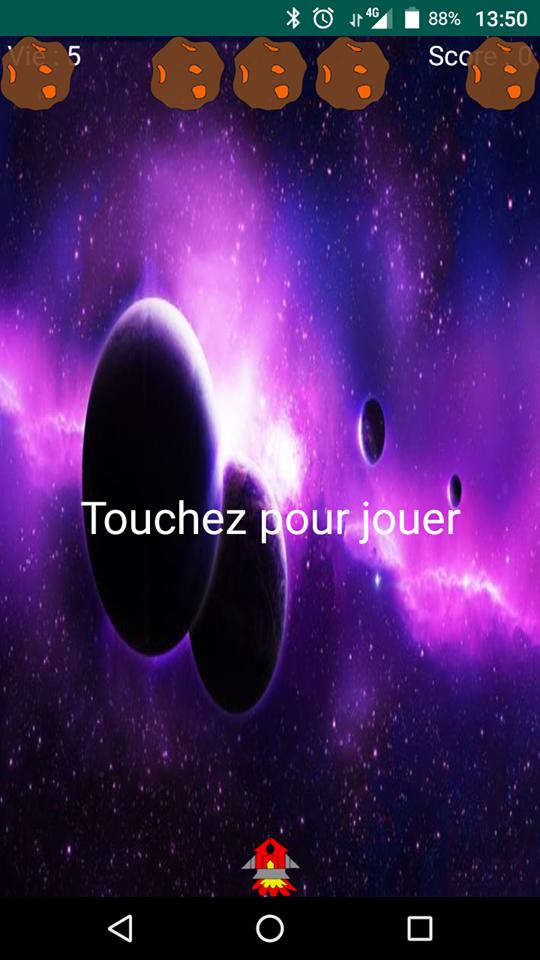
\includegraphics[scale=0.2]{BeforeGame.png}
\end{center}

Pour lancer le jeu sur Android, il suffit d'appuyer sur l'écran. (Petit piège les météores que nous voyons ne seront pas forcément à l'endroit où on les voit).
Sur IOS, le jeux commence dès que le bouton Commencer est appuyer.

\subsection{Le jeu}
\begin{minipage}[c]{.46\linewidth}
     \begin{center}
             \includegraphics[scale=0.2]{InGame.png}
         \end{center}
   \end{minipage} \hfill
   \begin{minipage}[c]{.46\linewidth}
    \begin{center}
            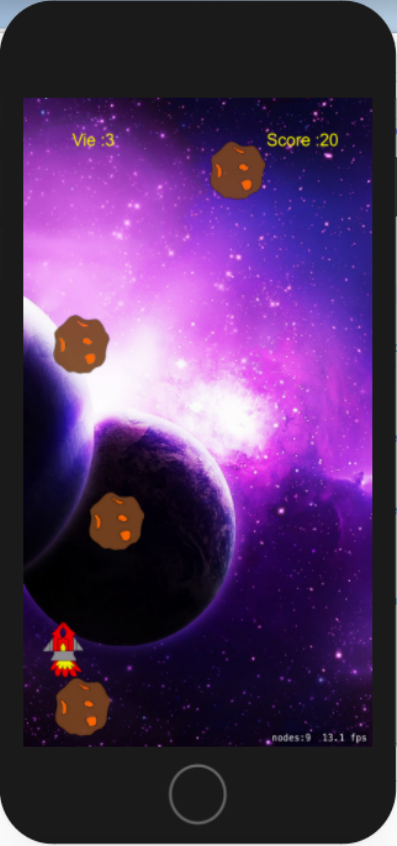
\includegraphics[scale=0.38]{InGameIOS.png}
        \end{center}
 \end{minipage}

Notre vaisseau va à droite ou à gauche jusqu'au bord respectif du téléphone, le joueur doit cliquer à droite ou à gauche de l'écran pour que le vaisseau change de direction, cependant le joueur ne pourra pas gérer la position exacte du vaisseau, il devra anticiper la vitesse des météores et du vaisseau pour ne pas se faire toucher.
La vie est affiché en haut à gauche de l'écran, avec 5 vie de départ et 1 vie en moins par contact avec un météore.
Le score afficher en haut à droite s'incrémente en fonction du nombre de météorite qui ne touche pas le vaisseau et qui arrivent jusqu'en bas de l'écran sous Android et en fonction du temps on gagne 5 points par seconde sur IOS. 
Les météores apparaissent de manière aléatoire en haut de l'écran et ont une vitesse aléatoire qui peuvent être égale ou différente rajoutant une difficulté surtout en début de partie pour le joueur sous Android. 
Sous IOS nous avons des météores possédant une vitesse identiques mais avec des temps d'apparition différentes.

\subsection{La fin du jeu (Game Over)}
\begin{minipage}[c]{.46\linewidth}
     \begin{center}
             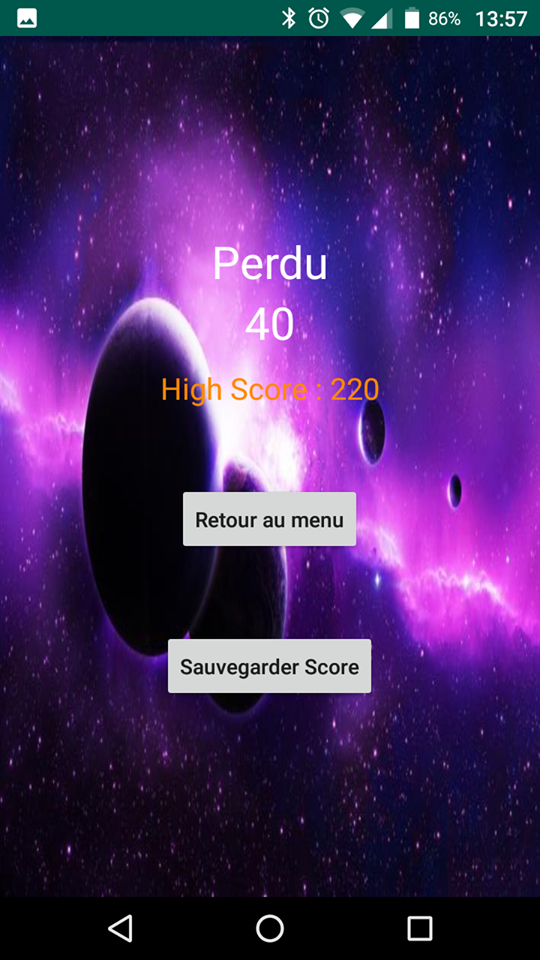
\includegraphics[scale=0.2]{GameOver.png}
         \end{center}
   \end{minipage} \hfill
   \begin{minipage}[c]{.46\linewidth}
    \begin{center}
            \includegraphics[scale=0.38]{GameOVerIOS.png}
        \end{center}
 \end{minipage}

Sur l'écran de fin, nous affichons le message de Game Over, le score et (sous Androïd) le High score soit le meilleur score que le jeu ait enregistré. 
Puis deux boutons nous invitent à retourner au menu ou sauvegarder le score que nous venons de réaliser.

\subsection{La sauvegarde}

\begin{minipage}[c]{.46\linewidth}
     \begin{center}
             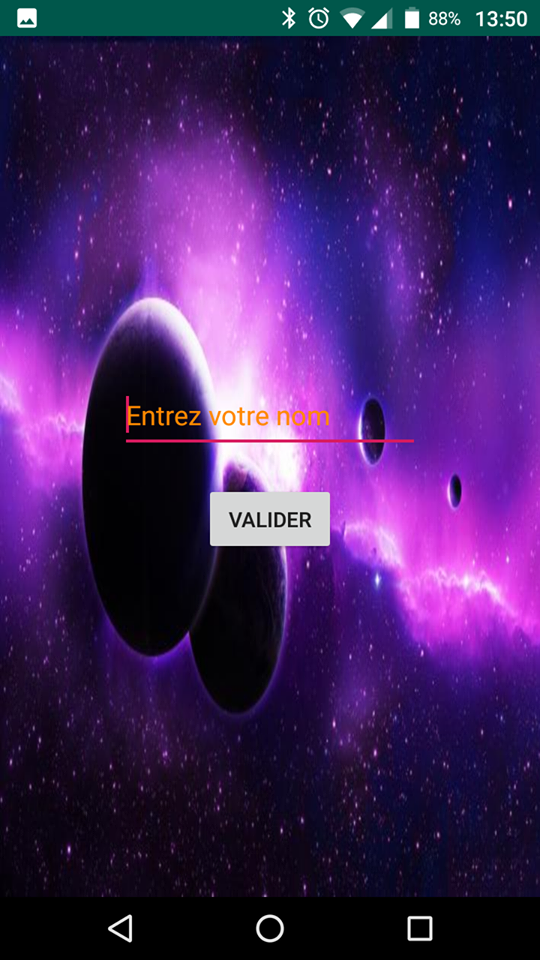
\includegraphics[scale=0.2]{SaveScore.png}
         \end{center}
   \end{minipage} \hfill
   \begin{minipage}[c]{.46\linewidth}
    \begin{center}
            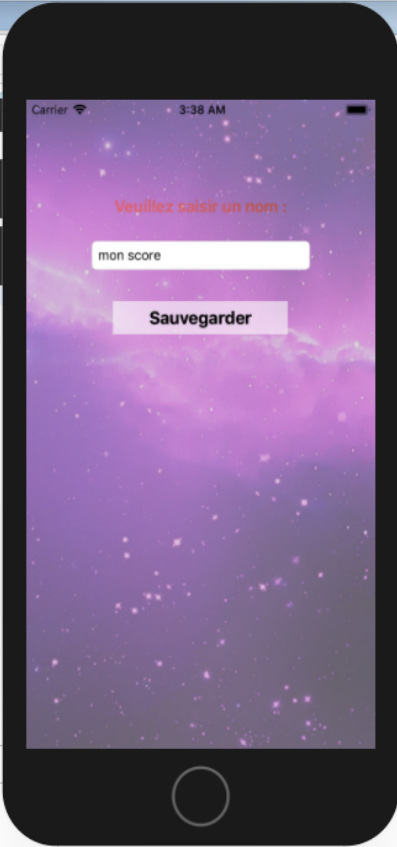
\includegraphics[scale=0.38]{SaveScoreIOS.png}
        \end{center}
 \end{minipage}

L'écran sauvegarde permet au joueur d'entrer son nom (ou pseudo) afin d'enregistrer son score en appuyant sur le bouton de validation.

\subsection{Présentation des scores}

\begin{minipage}[c]{.46\linewidth}
     \begin{center}
             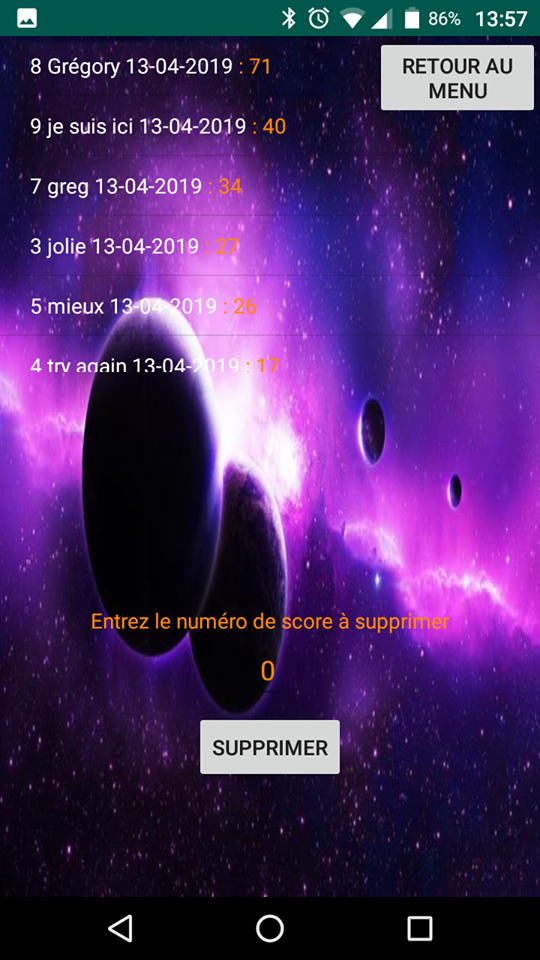
\includegraphics[scale=0.2]{AllScore.png}
         \end{center}
   \end{minipage} \hfill
   \begin{minipage}[c]{.46\linewidth}
    \begin{center}
            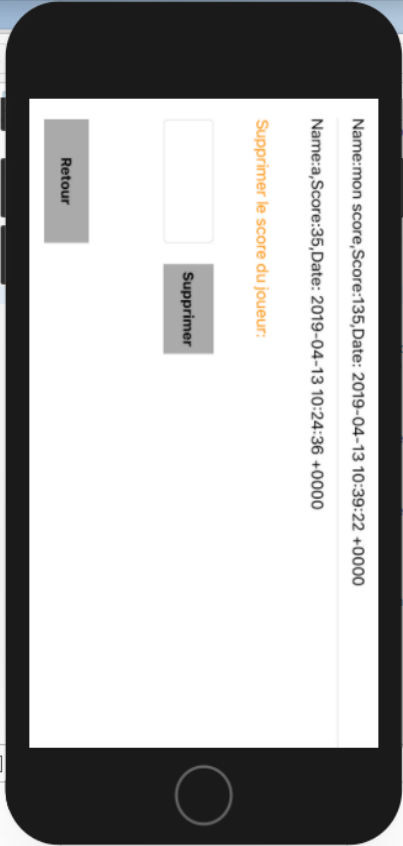
\includegraphics[scale=0.38]{tableauscoreIOS.png}
        \end{center}
 \end{minipage}

Le tableau des scores affiche tous les scores qui ont été enregistré sur le téléphone. Cet écran peut être vu en format portait ou paysage. Nous observons la possibilité donné au joueur de supprimer un score voulu, sous Android via le numéro de score affiché au début de l'affichage des scores ou sous IOS via le nom du joueur. 


\section{Le code}
Nous montrons dans cette section, quelques ligne de code phares de nos codes.

\subsection{Android}

\subsubsection{Les vues}
\textit{verbatim}:
\begin{verbatim}
 startActivity(new Intent(getApplicationContext(), MainActivity.class));
\end{verbatim}

Cette fonction permet de lancer une nouvelle vue (ici en l’occurrence la vue qui mène au jeu via le MainActivity.class).

\subsubsection{Collisions}
\textit{verbatim}:
\begin{verbatim}
if (vaisseau.getY() - Vaisseausize/2 <= meteorCenterY + Meteorsize/2
                && meteorCenterY - Meteorsize/2 <= vaisseau.getY() + Vaisseausize/2
                && vaisseauX - Vaisseausize <= meteorCenterX - Meteorsize/2
                && meteorCenterX - Meteorsize/2 <= vaisseauX + Vaisseausize)
\end{verbatim}

Afin de gérer les collisions, il faut vérifier le contact depuis le centre d'une image. Pour cela il y a quatre conditions, une par direction, à vérifier. Cela permet de partir d'un point à une ensemble de point qui fait l'image entière de notre vaisseau et du météore.

\subsubsection{Données envoyer entre vues}
\textit{verbatim}:
\begin{verbatim}
Intent intent = new Intent(getApplicationContext(), Scoring.class);
intent.putExtra("Score", score);     
startActivity(intent);
\end{verbatim}

Ce code montre le moyen de lancer une nouvelle vue via Intent, auquel nous rajoutons l'enregistrement d'une donnée (ici le Score) vers l'autre vue. La prochaine vue qui se lance (ici Scoring) aura comme donnée enregistré le score, qu'elle pourra ensuite utiliser en la récupérant grâce à :

\begin{verbatim}
s = getIntent().getIntExtra("Score", 0);
\end{verbatim}

Si il n'y a pas de valeur elle sera par défaut à 0.

\subsubsection{Toucher l'écran}
\textit{verbatim}:
\begin{verbatim}
if (me.getAction() == MotionEvent.ACTION_DOWN && me.getX() < ScreenWidth / 2)
\end{verbatim}

Le jeu se base essentiellement sur le toucher du joueur sur l'écran, cette fonction permet de voir si le joueur a appuyer sur l'écran et, ici en l'occurrence, si il a touché a gauche de l'écran grâce au me.getX(). 


\subsubsection{Enregistrement}
\textit{verbatim}:
\begin{verbatim}
 SharedPreferences sharedpreferences = getSharedPreferences("Save", Context.MODE_PRIVATE);
SharedPreferences.Editor editor = sharedpreferences.edit();
            editor.putInt("Hscore", s);
            editor.commit();
\end{verbatim}

Cce code permet d'enregistrer des préférences dans la vue. Nous l'utilisons pour enregistrer des valeurs (comme par exemple le HS qui est le High Score du jeu). Cette valeur, après avoir été enregistrer peut être obtenu sur cette vue grâce à :

\begin{verbatim}
 SharedPreferences sharedpreferences = getSharedPreferences("Save", Context.MODE_PRIVATE);
 int HS = sharedpreferences.getInt("Hscore", 0);
\end{verbatim}


\subsubsection{Comparer deux listes}
\textit{verbatim}:
\begin{verbatim}
class Sortbyroll implements Comparator<LesScores>
{
    public int compare(LesScores a, LesScores b)
    {
        return a.getScore() - b.getScore();
    }
}
\end{verbatim}

Cette classe permet de comparer deux valeurs dans deux listes. Cela permet ensuite de savoir quelle score est inférieur à l'autre pour permettre alors de trier les scores afficher. 



\subsubsection{Trier la liste}
\textit{verbatim}:
\begin{verbatim}
Collections.sort(scoring, new Sortbyroll());
Collections.reverse(scoring);
\end{verbatim}

Avec la bibliothèque Collections, nous pouvons trier la liste scoring dans l'ordre croissant tous d'abord (avec l'aide de la class précédemment vu). Puis nous inversons cette liste avec reverse car nous voulons l'ordre décroissant du score pour afficher le meilleur score en haut de la liste.

\subsubsection{Suppresion dans la liste}
\textit{verbatim}:
\begin{verbatim}
editor.remove("StringArrayElementNom"+ndele);
editor.remove("IntArrayElementScore"+ndele);
DateSE.remove("Date"+ndele);
editor.apply();
DateSE.apply();
\end{verbatim}

La suppression d'un score de la liste reviens a supprimer les valeurs qui se trouve dans le SharedPreferences et pour cela le SharedPreferences.Editor nous permet de supprimer des éléments de SharedPreference avec la fonction remove.

\subsection{IOS}

\subsubsection{Les vues}
\textit{verbatim}:
\begin{verbatim}
Storyboard: View, TabView, NavigationController etc
\end{verbatim}

Sous IOS les vues sont gérées par un fichier qui est Main.storyboard . C'est un outils graphique permettant la gestion de nos vues juste en les glissant dans la storyboard . Il y a différents types de View, nous pouvons avoir une simple vue View ou TableView pour faire une liste .Ci-dessous un exemple du fichier main.storyboard de notre jeux:

\begin{center}
	 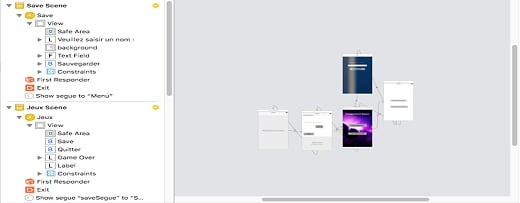
\includegraphics[scale=0.8]{storyboard.png}
\end{center}

\subsubsection{Collisions}
\textit{verbatim}:
\begin{verbatim}
 if contact.bodyA.node?.name == "player" || contact.bodyB.node?.name == "Meteor0"
 || contact.bodyB.node?.name == "Meteor1" || contact.bodyB.node?.name == "Meteor2"
 || contact.bodyB.node?.name == "Meteor3" || contact.bodyB.node?.name == "Meteor4" 
|| contact.bodyB.node?.name == "Meteor5"{

\end{verbatim}

Afin de gérer les collisions, tout ce passe dans la fonction  didBegin qui prends en paramètre un SKPhysicsContact . Dans notre projet nous avons utilisé une Collection appelé SKSprite ~\cite{raywenderlich} facilitant la détection de collision. Dans le code nous avons un objet A et un objet B et dans notre jeux A est représenté par le Joueur et B par les différentes Métorites.Lors d'une collision la vie du joueur est diminué et arrivé a 0 le score et la vie sont sauvegardés dans un protocol et une base de données que nous verrons ensuite.

\subsubsection{Données envoyer entre vues}
\textit{verbatim}:
\begin{verbatim}
Protocol afin de récupérer les données passés
protocol GameViewControllerDelegate: class {
    func GetScore(val: Int)
    func GetVie(val: Int)
}

    override func prepare(for segue: UIStoryboardSegue, sender: Any?) {
        if let destination = segue.destination as? PageSaveViewController {
            destination.score = Score
        }
    }
\end{verbatim}

Deux façons ont dû être utilisé afin de communiquer. Tout d'abord  via un Protocol entre la scène et son controller qui possède deux fonctions, une pour récupérer le score et l'autre pour la vie. Et enfin la méthode via la fonctions Prepare d'une vue à une autres

\subsubsection{Toucher l'écran}
\textit{verbatim}:
\begin{verbatim}
touchesBegan()
        if(locX > 0){
            if(player.position.x > w-89){player.position.x += 0 }
            else{
                player.position.x += 10
            }
        }else if (locX < 0){
            if(player.position.x < (-w + 89)){player.position.x += 0 }
            else{
                player.position.x -= 10
            }
        }

\end{verbatim}

Le jeu se base essentiellement sur le toucher du joueur sur l'écran comme étant annoncé dans la partie Android. Le déplacement utilise  la fonction touchBegan  récupérant les données X et Y lors du déplacement du doigts sur l'écran et sur l'actualisation de la position du joueur via le bloc if ci-dessus . Bien entendu ne voulant pas déplacer notre personnage sur l'axe Y nous avons gardé que la position X. 

\subsubsection{Enregistrement}
\textit{verbatim}:
\begin{verbatim}
        let appDelegate = UIApplication.shared.delegate as! AppDelegate
        let context = appDelegate.persistentContainer.viewContext
        
        let newUser = NSEntityDescription.insertNewObject(forEntityName: "Users", into: context)
        
        newUser.setValue(Date(), forKey: "date")
        newUser.setValue(TextField.text, forKey: "name")
        newUser.setValue(score, forKey: "score")
        
        do{
            try context.save()
\end{verbatim}

Le code ci dessus nous permet la sauvegarde de données comme par exemple ici la date courante, le nom , et le score. Les données enregistrées (dans le Core Data) peuvent être récupéré grâce au code ci dessous :

\begin{verbatim}
let request = NSFetchRequest<NSFetchRequestResult>(entityName:"Users")
        request.returnsObjectsAsFaults = false
        let sortDescriptor = NSSortDescriptor(key:"score",ascending: false)
        request.sortDescriptors = [sortDescriptor]
        
        do{
            let results = try context.fetch(request)
            if results.count > 0 {
                for r in results as![NSManagedObject]{
                    if let userDate = r.value(forKey: "date") as? Date , let userName = r.value(forKey: "name") as? String,let userScore = r.value(forKey: "score") as? Int{
                        arr.append("Name:\(userName)," + "Score:\(userScore)" + ",Date: \(userDate)")
                        print(userScore,userName,userDate)
                    }
                }
            }
\end{verbatim}

\subsubsection{Trier des données}
\textit{verbatim}:
\begin{verbatim}
        let sortDescriptor = NSSortDescriptor(key:"score",ascending: false)
        request.sortDescriptors = [sortDescriptor]
\end{verbatim}

Comme nous avons pu le voir dans le code précédent , nous avons effectué un tri selon le meilleur score via  la classe  NSSortDescriptor et nous avons appliqué cela au résultat d'affichage des données de la base.

\subsubsection{Suppresion dans la liste}
\textit{verbatim}:
\begin{verbatim}
-let appDelegate = UIApplication.shared.delegate as! AppDelegate     
 let context = appDelegate.persistentContainer.viewContext

-context.delete(object)
- try context.save()
\end{verbatim}

La suppression d'un score de la liste reviens a supprimer les valeurs qui se trouve dans le contexte  selon le nom d'un joueur.

\section{Conclusion}

Pour conclure, ce projet fut très enrichissant pour nous. La découverte de la programmation mobile sur IOS et Android nous montre des cas concret d'utilisation de code vu précédemment en 2ème année de licence. Nous avons pu remarquer de notable différence quand à la manière de programmer sur les types d'OS, en effet nous voulions montrer ses différences en codant le même jeu mais de manière différentes que nous proposer les OS utilisés. 
Les difficultés majeurs rencontrés auront été de savoir où placer tous les codes que nous voulions, la non acquisition de matériel Apple et des problèmes de gestion du Git sur Android Studio qui bugait assez souvent. 
Malgré cela, nous avons beaucoup apprécié faire ce projet et espérons que vous l'aurez tout autant apprécié que nous.

\subsection{Ressources utilisés:}
\begin{itemize}
\item Utilisation de la documentation de \textit{Java}~\cite{Javageek}
\item Utilisation de la documentation de \textit{SkSprite}~\cite{raywenderlich}
\item Utilisation de la documentation de \textit{Android}~\cite{developer}
\item Utilisation de la documentation de \textit{Apple}~\cite{AppDoc}
\item Aide obtenu pour des exemples d'utilisation sur les deux plateformes \cite{stackOverflow}

\end{itemize}
%%% La bibliographie:
\bibliographystyle{plain}
\bibliography{ma_biblio}
\	
\end{document}